Per gestire l'ambito multiplayer è stata realizzata un’architettura \textit{Client}-\textit{Server}.
Ogni giocatore è rappresentato dal \textit{Client} mente un unico \textit{Server} si occupa di gestire le varie connessioni con i \textit{Client} e lo stato delle partite.
\begin{center}
    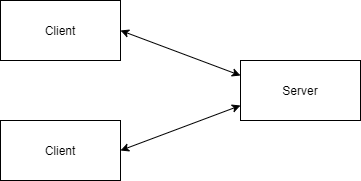
\includegraphics[scale=0.6]{architettura}
\end{center}
\subsection[Architettura]{Architettura}
\subsubsection{Core}
E’ stato poi realizzato, in maniera indipendente dalle altre componenti, un modulo di gioco che si occupa della sola gestione del gioco stesso, ovvero Machiavelli.
Esso definisce unicamente le entità base e le regole che lo caratterizzano.\newline \newline
Esso può essere considerato come se fosse un libreria esterna che non mantiene alcun stato relativo al gioco in corso, ma espone solamente delle API che possono essere utilizzate da chiunque. \newline \newline
Nel nostro caso è utilizzato sia dal \textit{Server} ma anche dal \textit{Client}: dal primo per gestire lo stato globale della partita ed aggiornarla in risposta alle mosse dei vari giocatori. Dal secondo per gestire internamente la fase del turno, validando le mosse effettuate, in cui l’utente può effettuare una quantità di mosse a piacimento interfacciandosi col core, per poi inviare al \textit{Server} il riepilogo delle azioni effettuate a fine turno.
Questo componente è stato realizzato integrando i linguaggi \textit{Scala-Prolog}.
\subsubsection{Server}
Il \textit{Server} è la componente principale del sistema, si occupa di gestire le connessioni con i \textit{Client} durante la fase di matchmaking, di creare le varie partite di gioco e di mantenere lo stato.
E’ diviso internamente in più componenti ed è costituito da 2 componenti principali:
\begin{itemize}
    \item \textit{LobbyManagerActor}: si occupa della gestione della lobby.
    È a lui che i Client chiedendo di giocare.
    Una volta raggiunte le condizioni necessarie per avviare una partita, genera un \textit{GameMatchManager} che si occuperà da quel momento in poi della gestione del gioco.
    \item \textit{GameMatchManagerActor}: si occupa di gestire una partita in corso.
    In fase di runtime ne saranno presenti molteplici attivi contemporaneamente, uno per ogni partita.
    Mantiene lo stato della partita corrente e gestisce i turni di gioco, ricevendo le azioni da ogni utente e comunicando a tutti gli altri ogni aggiornamento avvenuto.
\end{itemize}
\subsubsection{Client - MVC}
É utilizzato dall’utente per poter cercare una partita secondo le proprie preferenze e per giocare la stessa.
Internamente realizzato seguendo il pattern MVC, è poi ulteriormente diviso in due macro parti che rispecchiano all’incirca quello già visto sul \textit{Server}:
\begin{itemize}
    \item Una di gestione della fase iniziale di gioco, ovvero la lobby, utilizzata per poter ricercare la partita desiderata;
    \item Una di gestione del gioco stesso, utilizzata nel momento in cui la partita è in esecuzione, con cui l’utente può effettuare mosse durante il proprio turno, comunicarle al server e ricevere gli aggiornamenti conseguenti alle azioni effettuate dagli altri giocatori.
\end{itemize}
\subsubsection{Comunicazione client-server}
Tra il \textit{Client} e il \textit{Server} si è scelto di utilizzare un modello di comunicazione a scambio di messaggi, realizzata grazie all’utilizzo del framework \textit{Akka}.
Questa scelta ha permesso di gestire ad alto livello le comunicazioni tra le componenti senza preoccuparsi dei dettagli implementativi della comunicazione stessa.
\subsubsection[Flussi di interazione]{Flusso di interazione client server}
Il grafico seguente riassume gli aspetti visti in precedenza nei paragrafi relativi alla parte \textit{Client} e \textit{Server}, mostrando come la parte del flusso di gioco del turno del giocatore venga gestito completamente in locale, mentre il \textit{Server} viene contattato solo al termine per validare le mosse effettuate dal giocatore e inviare lo stato aggiornato a tutti gli altri.
\begin{center}
    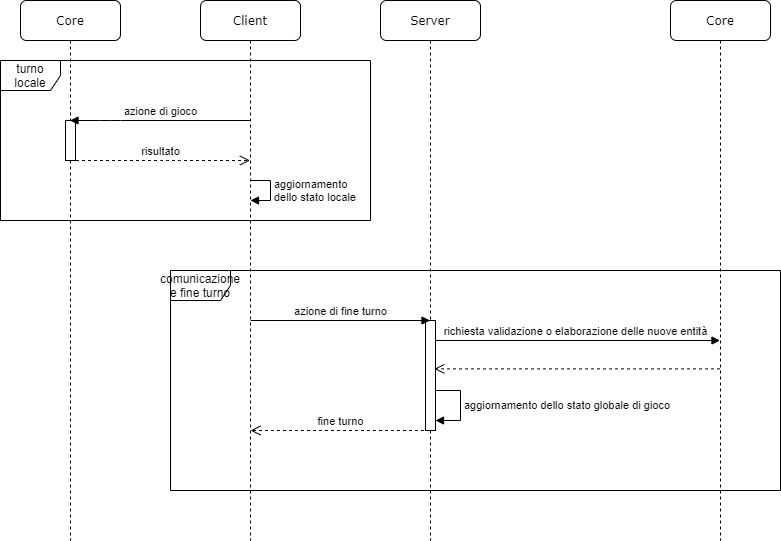
\includegraphics[scale=0.5]{flusso-interazione-client-server}
\end{center}
Questa scelta è stata fatta per garantire ottime prestazioni durante il gioco.
La fase del turno è infatti quella caratterizzata dalla frequenza più elevata di interazioni utente (riposizionamento carte, ordinamento della carte in mano, annullamento delle mosse precedenti ecc..), tutte operazioni non di rilevanza per gli altri giocatori connessi, a cui interessa più che altro lo stato finale del turno dell’avversario.
Il sistema è stato comunque modellato in maniera tale da prevedere modifiche future anche sotto questo aspetto, in maniera da spostare tutto lato server o lato client a seconda delle esigenza (ad esempio in una modalità singolo giocatore vs AI).
\newpage